\section{Experimental results}

\subsection{Dataset preprocessing}

The dataset in use is the Illinois Bulk Dataset, that contains 
183146 cases with 194366 judges opinions. 

The first step of the preprocessing is to merge the opinions about a 
case into one, obtaining a single document for each dataset entry.  
Then, each document goes through a text cleaning and tokenization phase, 
where the first part is done with the help of regular expressions, 
while the second uses Spacy to obtain a list of terms.

\subsection{Word of interest expansion}

The project started with a collection of relevant words for three categories, 
namely weapons, narcotics and investigations. The idea is to preserve these words
in each preprocessing phase, especially when filtering out words 
that do not meet a required frequency in the dataset. 
To have a better set of interesting words to keep we opted to expand them 
using pre-trained word embeddings, the \emph{GoogleNews} models.
The process consists of finding similar words for each word 
of interest, checking that these words are in the dataset, 
with a manual final review to remove unnecessary or wrong words.

\subsection{Topic modelling}

To have an overview of the topics discussed on the dataset a Latent 
Dirichlet Allocation model is trained on the tokenized texts.
One of the key parameters of such a model is the number of topics, and, 
given the fact that cases could potentially talk about anything, an 
\emph{Halving search} is performed to find a good value.

We opt for an halving search since the number of topics could be anything, 
we fixed a range between ten and thirty and training each model 
to then evaluate results would take a huge amount of time. Halving search 
mitigates the problem, as it trains firstly on smaller datasets, select 
the best models, and retrain on bigger slices of data until a final model 
is found. This methodology can be ten times faster then grid search. 
The selection criterium for the search is the Log Likelihood of each model.
The search revealed that the optimal number of topics is 14.

The resulting topics are promising but the words of interest, namely a collection 
of narcotics, investigation and weapons terms, are merged together in a few topics.
\begin{figure}
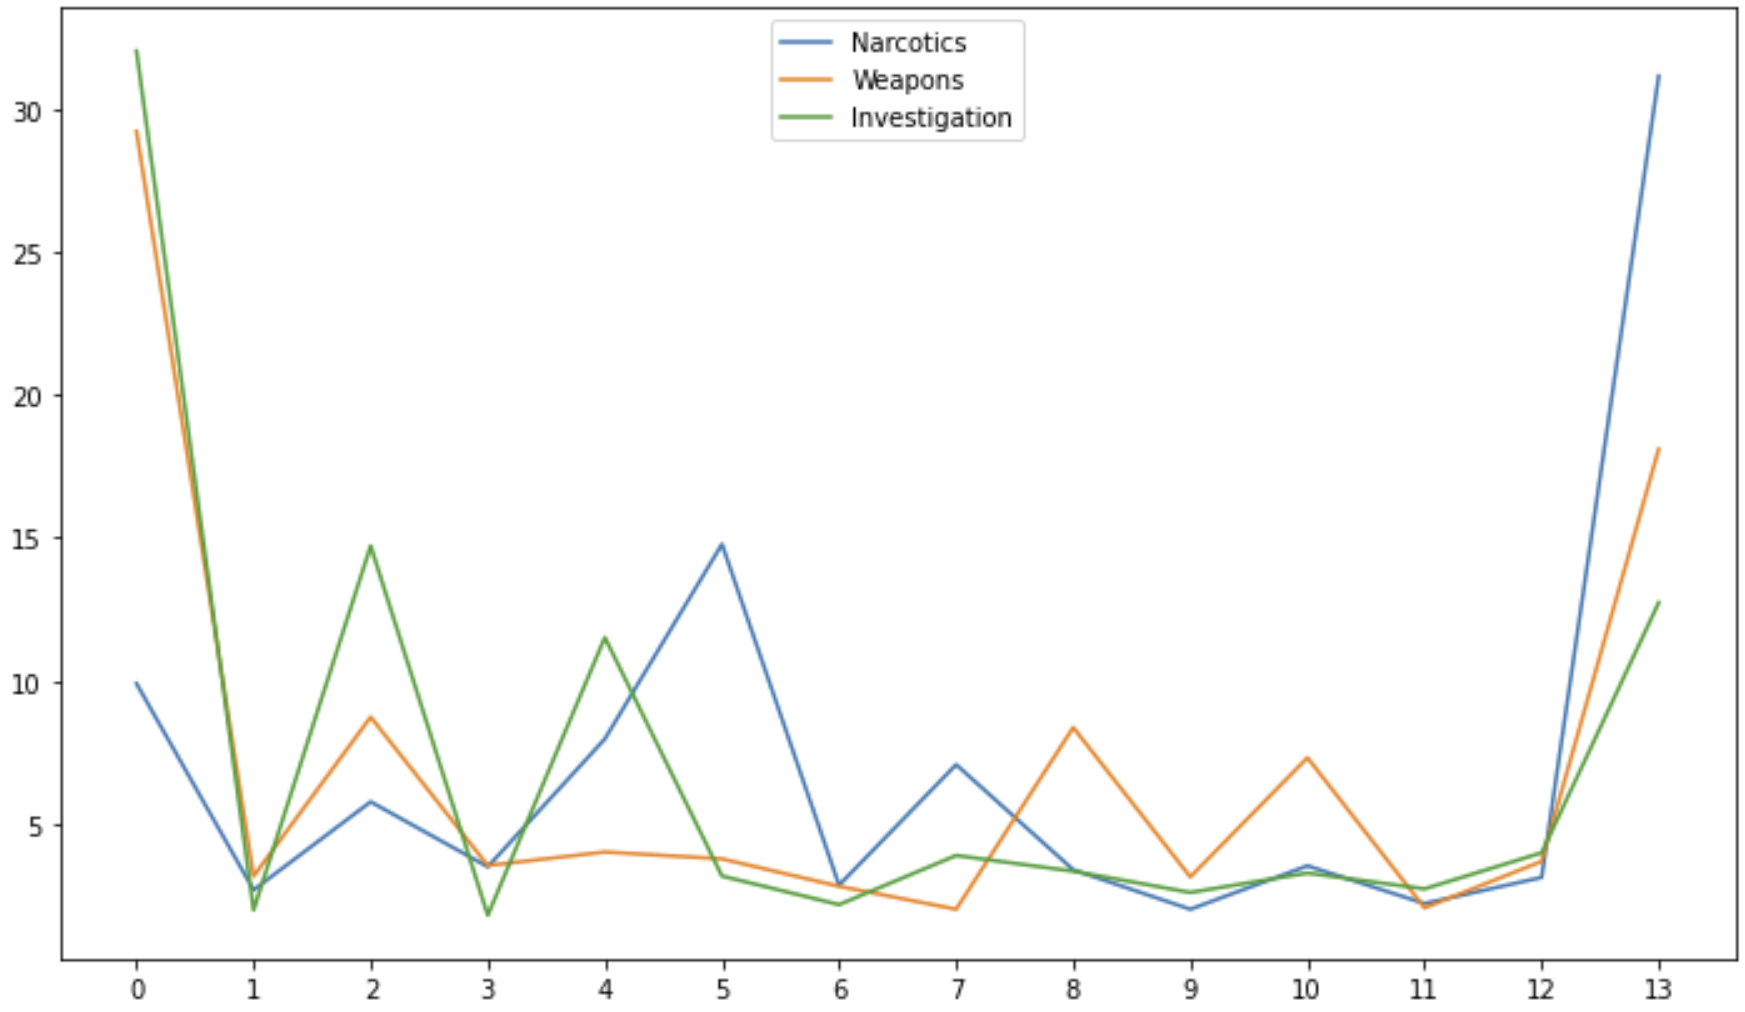
\includegraphics[width=\textwidth]{images/topic_distribution.png}
\caption{Sets of interest distributions on generic topics} \label{fig1}
\end{figure}
To solve the issue we decide to run topic modelling on a subset of the previous 
topics with the same technique as before. The result is similar, we find again 14 topics, 
but this time they are much more specific.

\subsection{Temporal word embeddings}

One of the objective of the project is to find correlations among words and one tool 
that can be used is word embeddings. The technique assigns a real vector of a given dimensions
to each word in the document collection, creating a way to directly compare the context 
similarity between two terms.

For this task we used Gensim's Word2Vec implementation and trained different models 
in three ways:
\begin{enumerate}
    \item \emph{Global model}: trained on the entire document collection, with 100 components vectors;
    \item \emph{One year models}: they are trained on subsets of the dataset divided by years;
    \item \emph{Ten years models}: trained on epochs of 10 years each.
\end{enumerate}
The first model gives information about the whole dataset, it can be used to compute 
similar words queries, while the others can be exploited to find context and semantic shifts 
among the temporal axis.
Taking inspiration from the HistWords~\cite{hist-words} work on semantic shift, we start by aligning the models, 
and then find, given a word and a base year, the similarity of that word in time with respect 
to the base year. This approach can reveal if a word changed semantic or context, and when, 
with respect to a given year, an example can be seen in \vref{fig2}.

Similarly, the ten year models are aligned, but this time, given a term, we compute the 
difference among two consecutive epochs. The idea is similar to the previous one but slightly 
different, this time a drop in the similarity sequence 
reveals a change of meaning from an epoch to the other, the resulting 
sequence can be seen in \vref{fig3}.

\begin{figure}
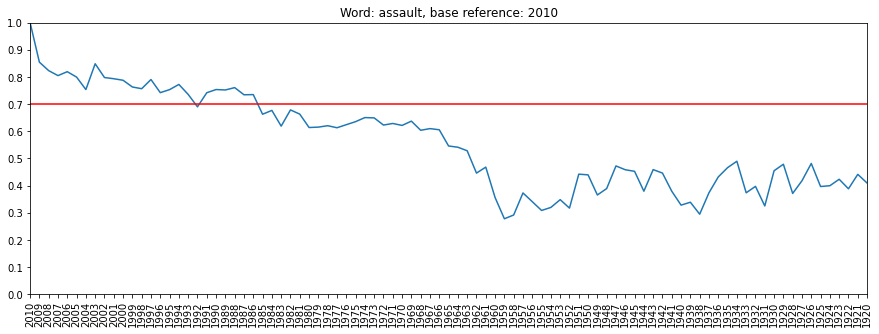
\includegraphics[width=\textwidth]{images/semantic_1.png}
\caption{Semantic shift of the word assault 
with respect to the year 2010, we can see a drop if similarity around 1960.} \label{fig2}
\end{figure}
\begin{figure}
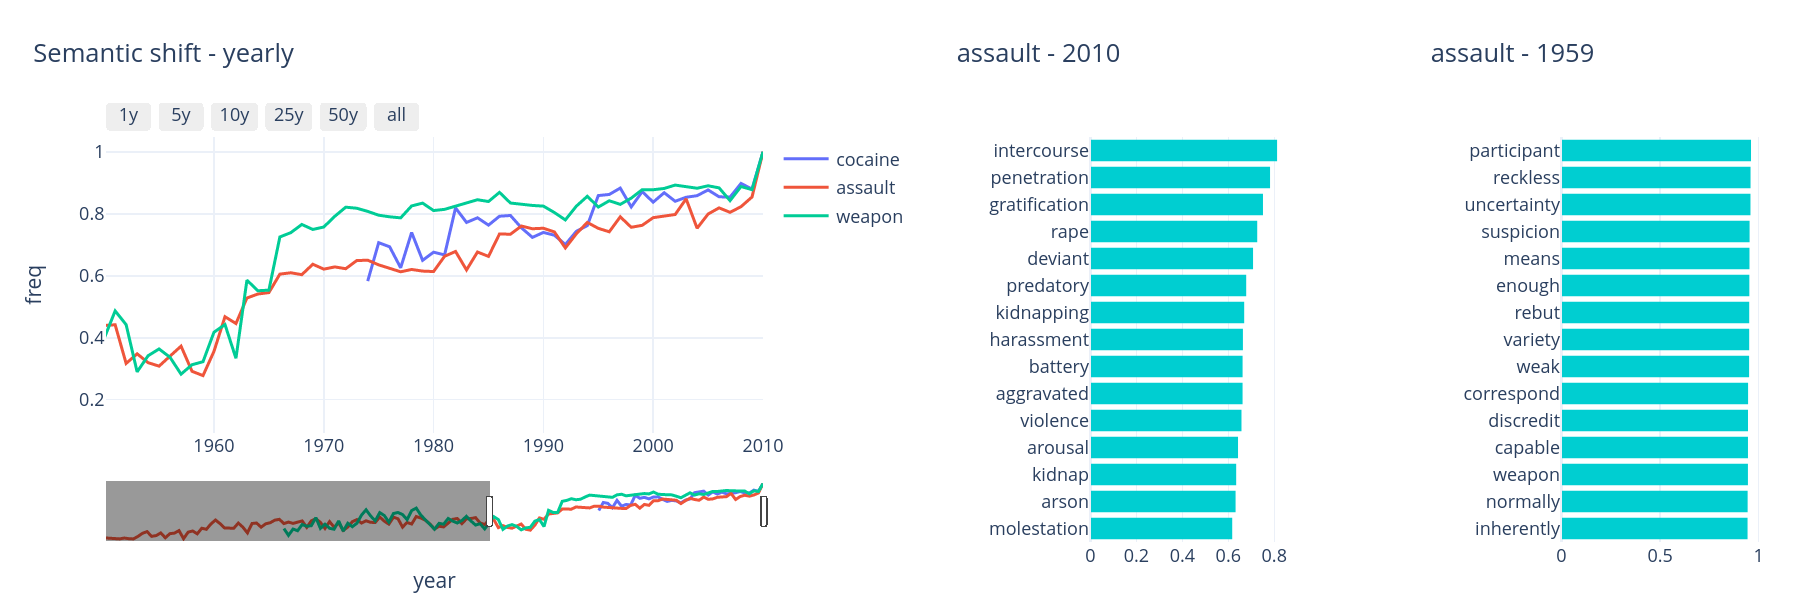
\includegraphics[width=\textwidth]{images/semantic_2.png}
\caption{Similarity between consecutive epochs of the term assault, we can see a 
drop between 1980-1970 and 1970-1960.} \label{fig3}
\end{figure}

\subsection{Webapp}
In order to visualize and explore the results of the analysis, a web interface has been developed. Through the UI, the
user can search multiple words united (separated by ",") and/or compare words (separated by "-"); the app will show
various interesting sections, one focused on the analysis of the searched words (\vref{fig4}) and one on the
analysis of a selected topic (\vref{fig5}):
\begin{itemize}
  \item Top 15 words of similar context of the searched words (using word embeddings).
  \item Frequency graph of documents in time containing the searched words.
  \item Semantic shifts of the searched words, both by epoch (two adjacent epochs of 10 years) and by single year.
    If the user clicks on a point of the graph, the contexts of the selected word in the different selected years/epochs
    will be showed, allowing the comparison of contexts which helps understanding the evolution of words meaning and usage
    during time.
  \item Topic distribution of the searched words (both generic and areas of interest-specific topics). By clicking on the
    showed radar chart, or on the lateral list of topics, the selected topic info will be loaded in the below section.
  \item Most important words of the selected topic. There are three ways of visualization: a barchart with the first 15
    words, a Wordcloud with the first 80 and a Treemap with the first 50.
  \item Topic distribution over time and over the different Illinois courts.
\end{itemize}
The application has been developed in Python and is accessible at
\url{https://illinois-cases-analysis-webapp-qka7d4ktba-ew.a.run.app/}.
\begin{figure}
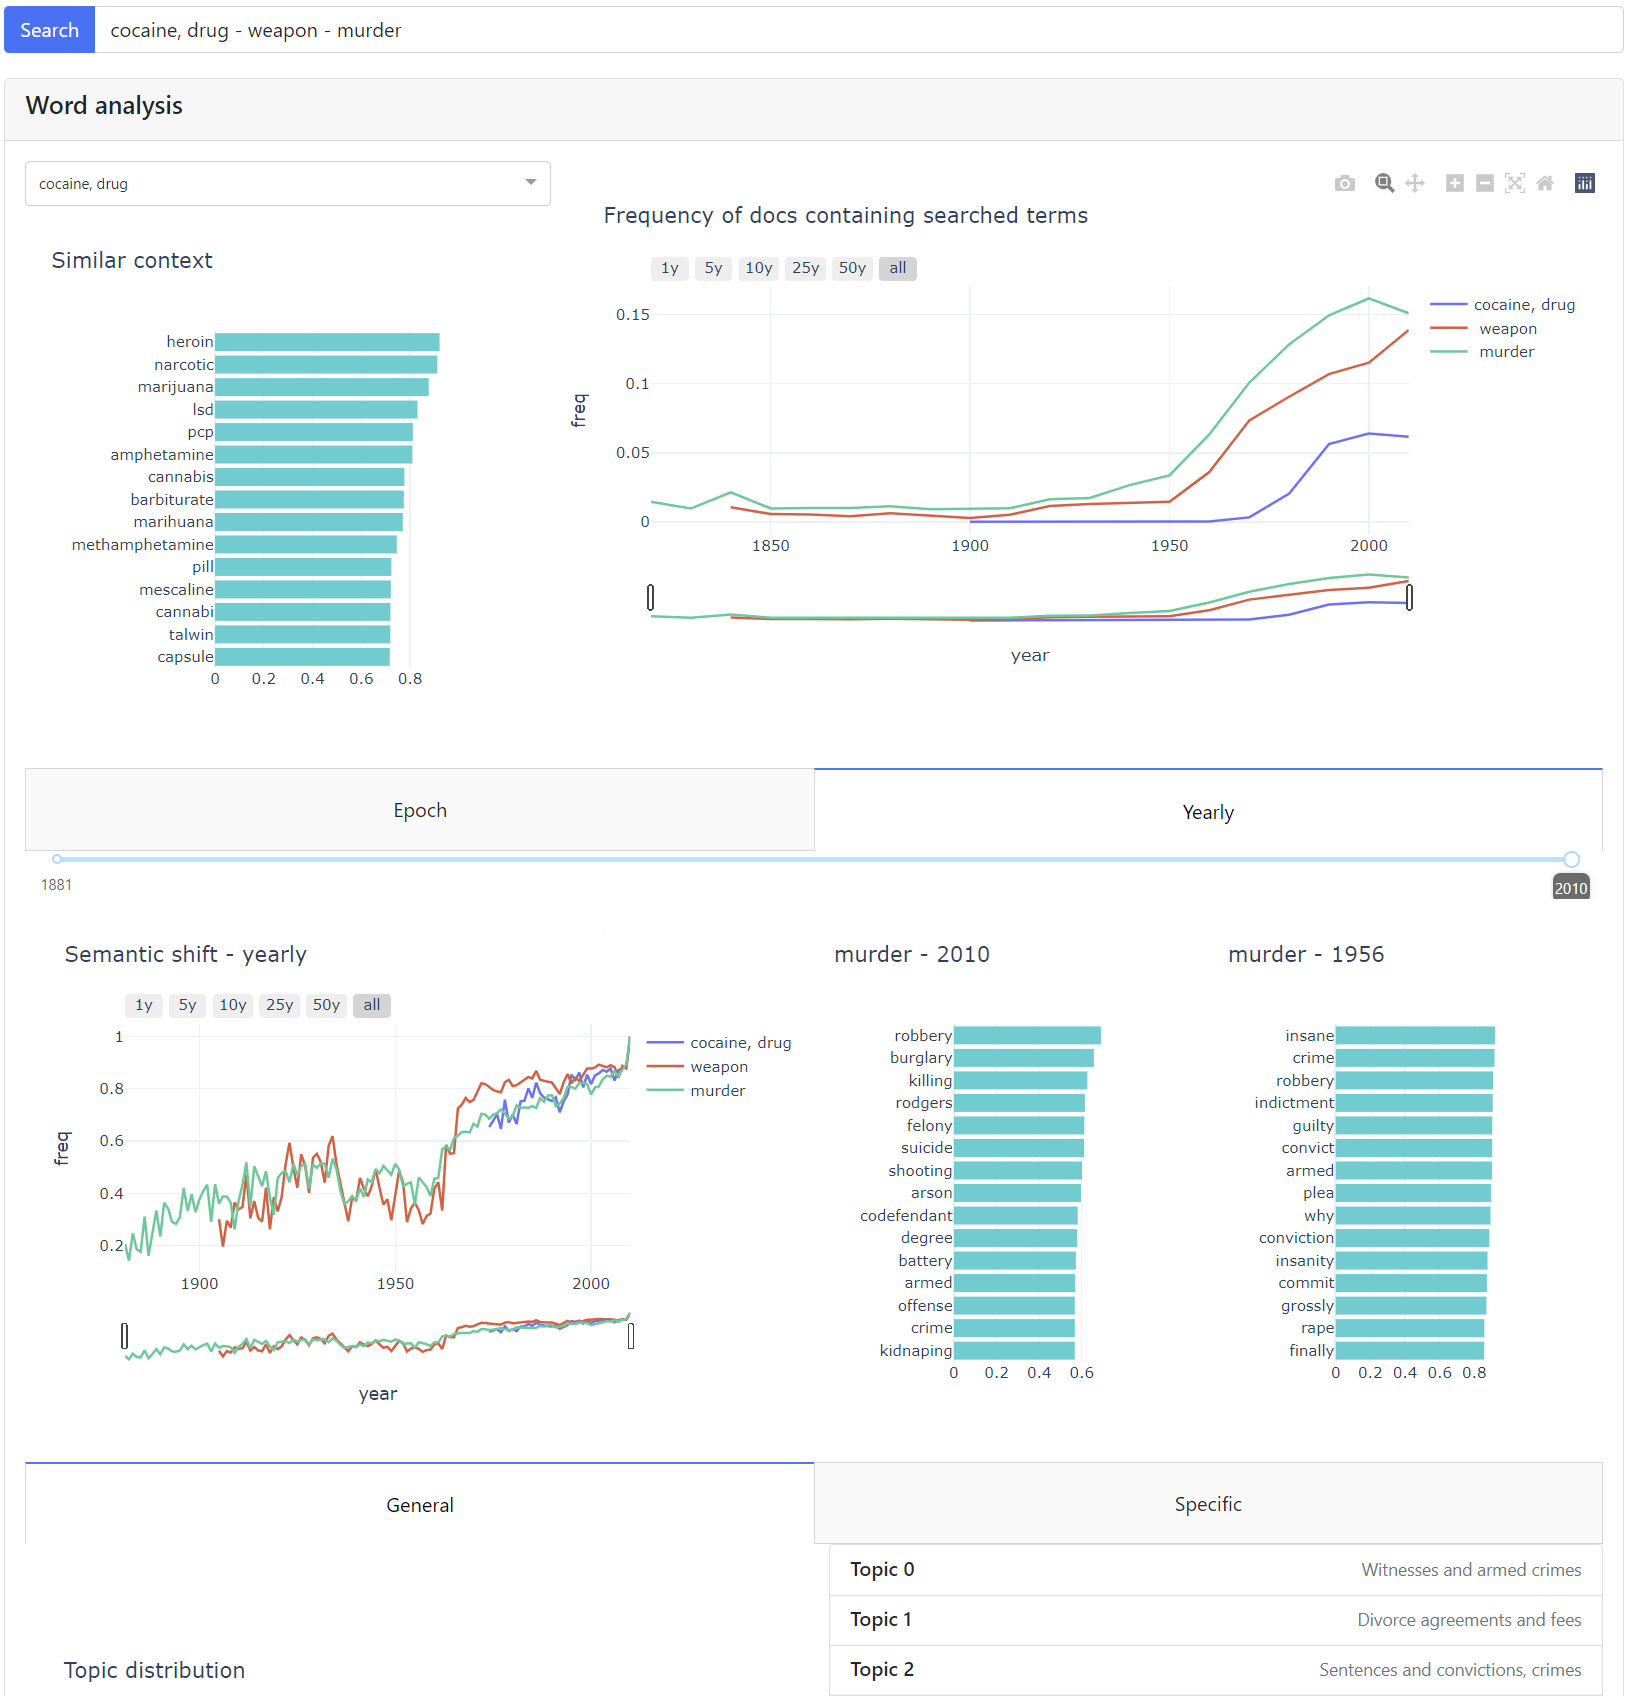
\includegraphics[width=\textwidth]{images/webapp.png}
\caption{Searched words analysis} \label{fig4}
\end{figure}
\subsubsection{Webapp developing technology}\hfill\\
In order to fastly create an interesting interface, three python-based frameworks for web developing have been considered:
\begin{itemize}
    \item Voila and ipywidgets. Because the whole project has been developed using Jupyter notebooks, it would have
    been natural to develop the webapp in a new notebook. ipywidgets allow to create dynamic elements and behaviour to
    a Jupyter Notebook, while Voila allows to have better design and the possibility to run the notebook as if it was
    a web page (hiding all the code and markdown of the notebook itself).
    \item Dash. It consists in a point-&-click interface to models written in Python, vastly expanding the notion of
    what's possible in a traditional "dashboard." It is the main solution for data scientists and engineers in order to
    put complex Python analytics in the hands of business decision-makers and operators.
    \item Streamlit. Similar to Dash.
\end{itemize}
Voila and ipywidgets have been discarded because of the technical requirements needed to run and understand a Jupyter
notebook; even if the complexity could have been partially hidden, the graphics component of ipywidgets are not so
captivating as it would have been required from a website which main goal was to be easy to use and undestand, while
providing a nice design.

Dash and Streamlit are really similar one to another, with both offering beautiful interfaces easy to deploy. Dash has
been chosen because of its popularity and presence in the data science applications world, but Streamlit is quite new
but in the last years it has gained a lot of popularity and attention.

In all three frameworks (and particularly in Dash), the workflow is pretty similar; the design elements of the UI are
defined in an HTML-style using the framework Python libraries predefined classes, while the user-generated events are
captured using callback functions, which connect the input elements (e.g. a button which has been clicked) to output
elements (e.g. a graph), defining the required processing and manipulation of output elements.
\begin{figure}
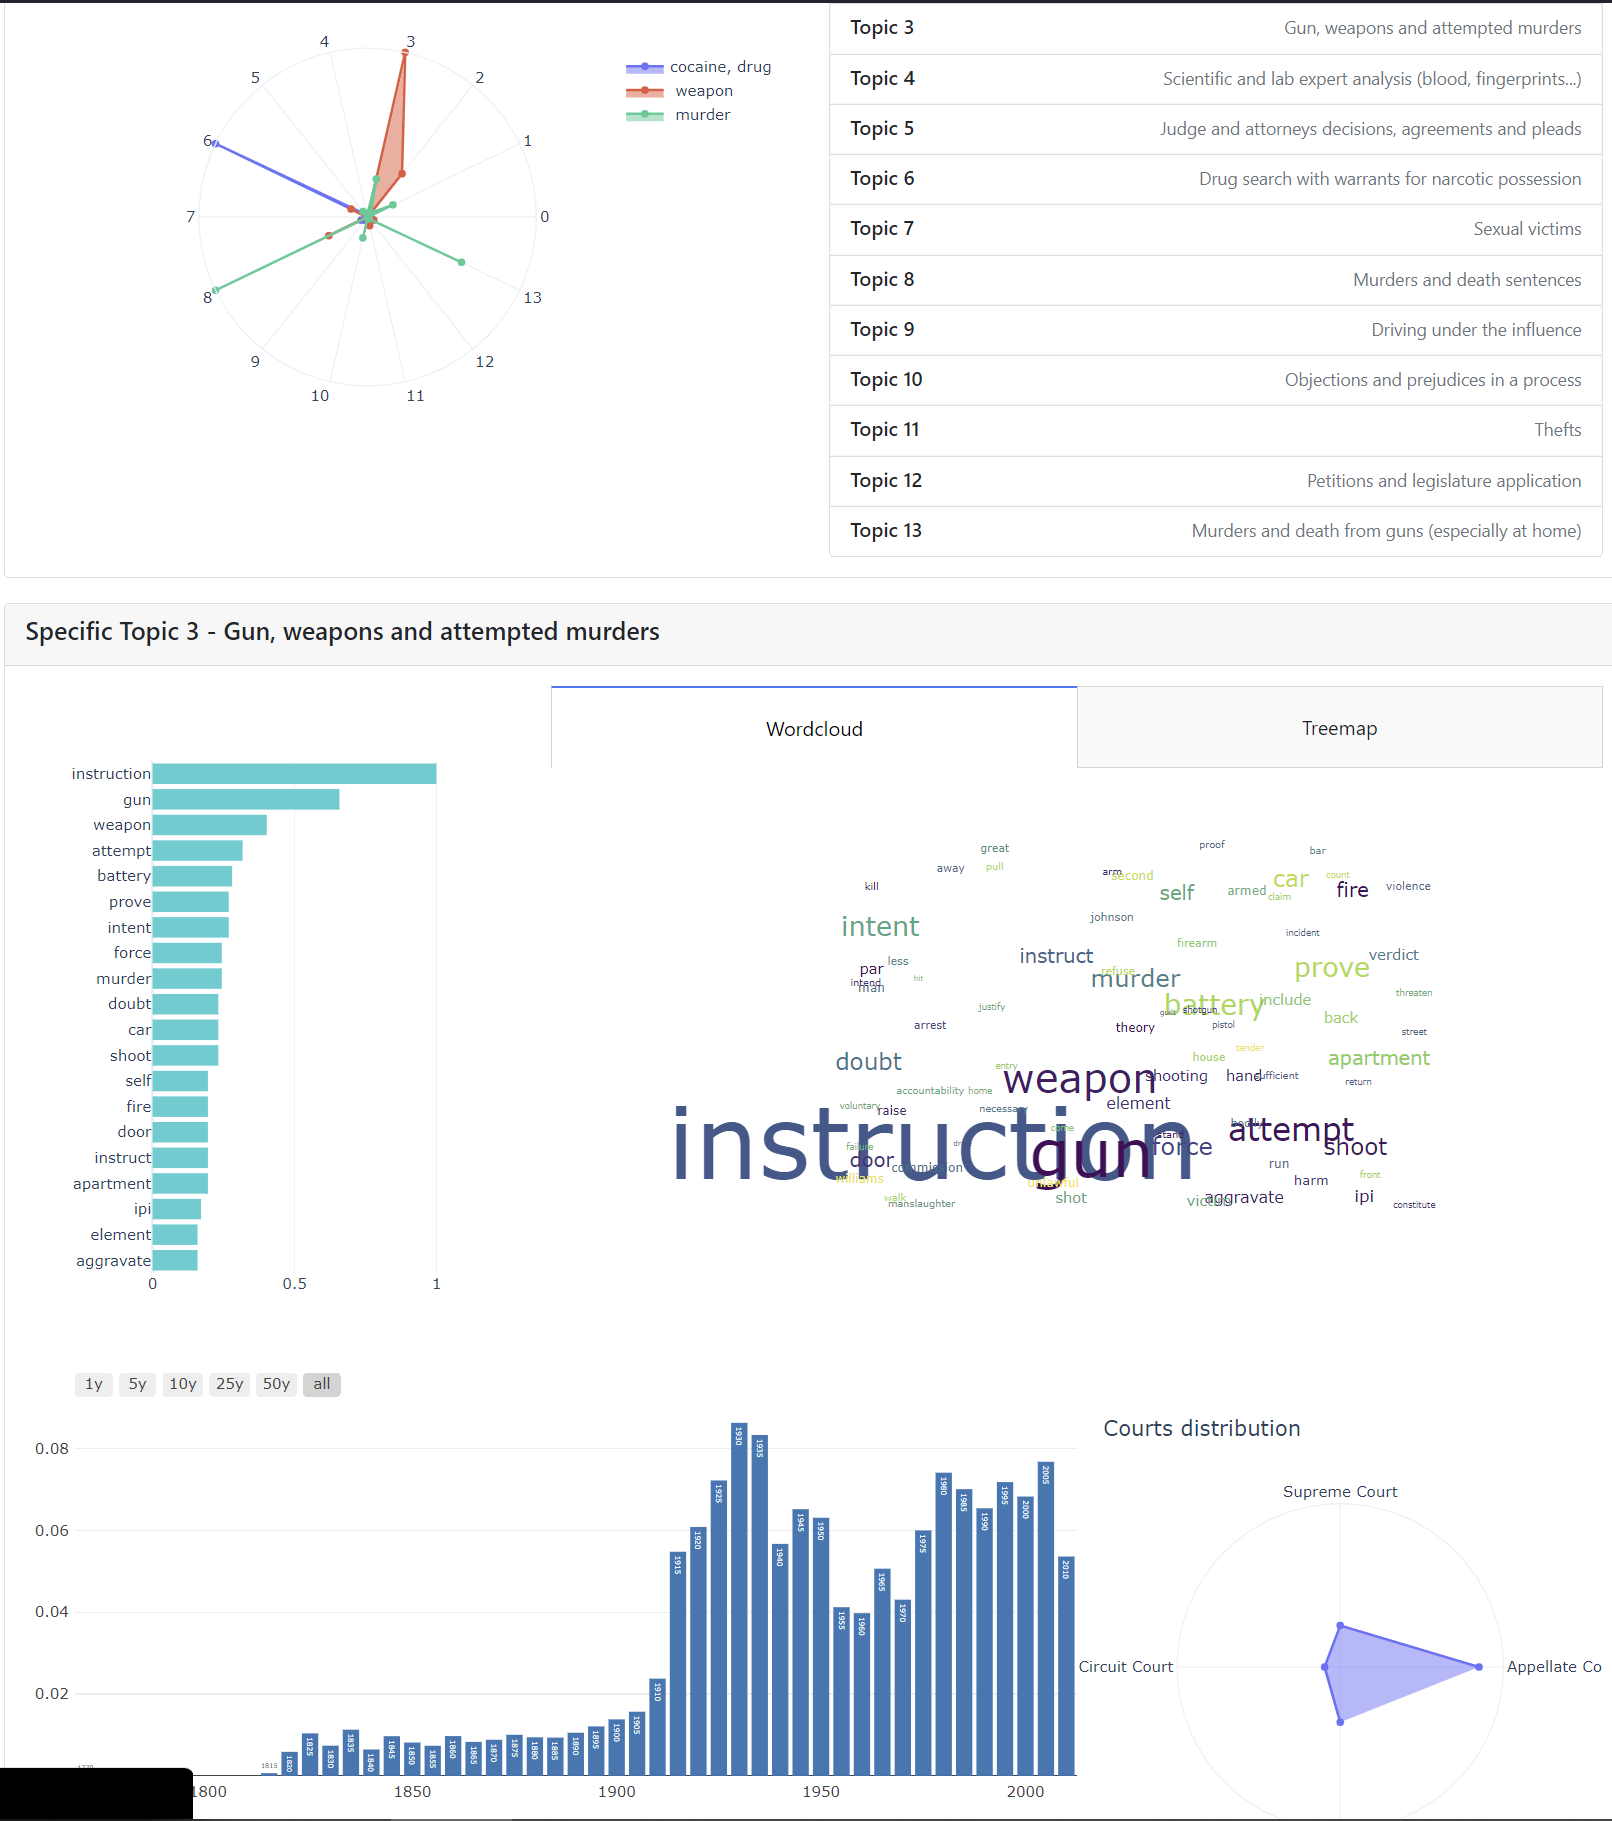
\includegraphics[width=\textwidth]{images/webapp2.png}
\caption{Selected topic analysis} \label{fig5}
\end{figure}
\subsubsection{Cloud hosting}\hfill\\
Because the developed prototype has many interested features which could be already interesting to explore, it has been
decided to publish it on a public domain, in order to make it easily accessible and usable to anyone who could be
interested in it, without any technical requirement.

Firstly, many free-to-use hosting sites of Python web applications have been tested, such as PythonAnywhere, Heroku...,
but all of them allowed a tiny free tier (at maximum, 1 GB of disk). Because of the large data that it is used to
show the various statistics (only the word embeddings files, divided by temporal periods, take up 5 GB), it was not
possible to use any of them.

Google Cloud Platform has been chosen to host the webapp. In order to do so, a Docker image has been created, starting
from the directory of the webapp. The image has been sent to Google Cloud through a build phase which created an online
container of 16GB of memory and 4 CPUs (the last and only combination allowed which permitted also to load all the
required files). In this way, by using Cloud Run, the webapp is officially a running service which can be accessed at
\url{https://illinois-cases-analysis-webapp-qka7d4ktba-ew.a.run.app/}.\\
Google Cloud offers a huge Free Tier, but because of the highest possible configuration chosen (the only one working),
it is still be expected to spend around \$3 per month. Most importantly, the container instance is active only during the
period in which requests are served; this means that, if no other instance is active, the container has to be launched
from an idle state, taking even up to around 3/4 minutes to be accessible (due to the huge amount of files that it
has to load in order to make all the analysis functionality available, especially word embeddings).